\documentclass{standalone}
\usepackage{tikz}
\usepackage{ctex,siunitx}
\setCJKmainfont{Noto Serif CJK SC}
\usepackage{tkz-euclide}
\usepackage{amsmath}
\usetikzlibrary{patterns, calc}
\usetikzlibrary {decorations.pathmorphing, decorations.pathreplacing, decorations.shapes,}
\begin{document}
\small
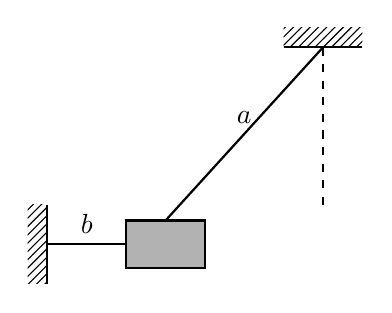
\begin{tikzpicture}[>=stealth, thick]
  % \useasboundingbox(-1,-0.75)rectangle(3.7,1.4);
  \fill [fill=black!30, draw] (2,0.2) rectangle (3,.8);
  \draw (2,.5)--(1,.5)node[midway,above]{$b$};
  \fill [pattern = north east lines] (0.75,0) rectangle (1,1);
  \draw (1,1)--(1,0);
  \fill [pattern = north east lines] (4,3) rectangle (5,3.25);
  \draw (4,3)--(5,3);
  \draw [dashed] (4.5,3)--(4.5,1);
  \draw (4.5,3)--(2.5,.8)node[midway,above]{$a$};
  \end{tikzpicture}
\end{document}